\documentclass[11pt]{amsbook}

\usepackage{../HBSuerDemir}

\newcommand{\uvec}[1]{\boldsymbol{\textbf{#1}}}

\begin{document}
    	
\hPage{b2p1/239}

\subsubsection{Curvature of plane curves} 
Let 
$$ 
	r : r(x) = x \uvec i + y \uvec j, \quad y=f(x)
$$
be a plane curve.
\begin{align*}
	r'(x) =\ & (\uvec i + y' \uvec j) \ \tfrac{\hDif x}{\hDif s} \ (\text{with  } \hDif s = \sqrt{1 + {y'}^2} \hDif x) \\
	=\ & (\uvec i + y' \uvec j) \quad \tfrac{1}{\sqrt{1 + {y'}^2}} \\
	r''(x) =\ & [(y'' \uvec j)] \tfrac{1}{\sqrt{1 + {y'}^2}} - (i+y' \uvec j) \tfrac{y' y''}{{(1 + {y'}^2)}^{3/2}}] \quad \tfrac{1}{\sqrt{1 + {y'}^2}} \\
	=\ & [ -\tfrac{y'}{1 + {y'}^2} \uvec i + (1 - \tfrac{{y'}^2}{1+{y'}^2}) \uvec j ] \tfrac{y''}{1 + {y'}^2}  \\
	=\ & (-y' \uvec i + \uvec j) \quad \tfrac{y''}{{(1+{y'}^2)}^2} \\
	K^2 =\ & (1+{y'}^2) \tfrac{{y''}^2}{{(1+{y'}^2)}^4} = \tfrac{{y''}^2}{{(1+{y'}^2)}^3} \\
	K =\ & \pm \tfrac{{y''}^2}{{(1+{y'}^2)}^{3/2}} \Longrightarrow \rho = \tfrac{{(1+{y'}^2)}^{3/2}}{{|y''|}}
\end{align*}
For a plane curve the curvature has the equivalent definition. namely


\begin{figure}[htbp]
\begin{minipage}{0.45\linewidth}
	\begin{align*}
		K = \frac{\hDif \alpha}{\hDif s} 
	\end{align*}
\end{minipage}
\begin{minipage}{0.45\linewidth}
	\centering
	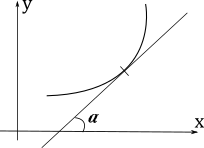
\includegraphics[width=0.65\textwidth]{images/b2p1-239-fig01}
\end{minipage}
\end{figure}

\par 
Indeed,

\begin{align*}
	\tan\ \alpha = y' \Rightarrow \alpha = \arctan y' \Rightarrow \frac{\hDif \alpha}{\hDif s} = \frac{y''}{1+{y'}^2}  \frac{\hDif x}{\hDif s} \\
\end{align*}
\begin{align*}
K = \frac{\hDif \alpha}{\hDif s} =  \frac{y''}{1+{y'}^2}  \frac{1}{\sqrt{1+{y'}^2}} =  \frac{y''}{{(1+y')}^{3/2}} \text{.}
\end{align*}
\end{document}